\subsection{課題3}
\ref{subsec:report-2}で求めた$k_{x_m}$、$k_{y_m}$の誤差を定量的に考察する。

$N_A$は、$N_A=R/k$であるから、$k$を用いて考える。
$k_{x_m}$、$k_{y_m}$それぞれ相対誤差は次のようになる。
\begin{align}
    \delta k_{x_m} & = \dfrac{\left| k_{x_m} - k \right|}{ k_{x_m} } \nonumber \\
                   & = \SI{55.5}{\percent}                                     \\
    \delta k_{y_m} & = \SI{31.9}{\percent}
\end{align}

まず、$k$と$T$の関係を考える。
$\eta$は表\ref{tab:water-viscosity}のように温度依存性があり、$k$も\ref{eq:brownian-motion}式から温度を含む。
$T$は溶液の温度であるが、実際に計測したのは室温である。
したがって、室温と溶液の温度の差が誤差の一因として考えられる。
$\eta$と、$k$の$T$依存性は次の\ref{fig:k-n-relation}のようになる

\begin{figure}[htbp]
    \centering
    \begin{minipage}[b]{0.45\linewidth}
        \centering
        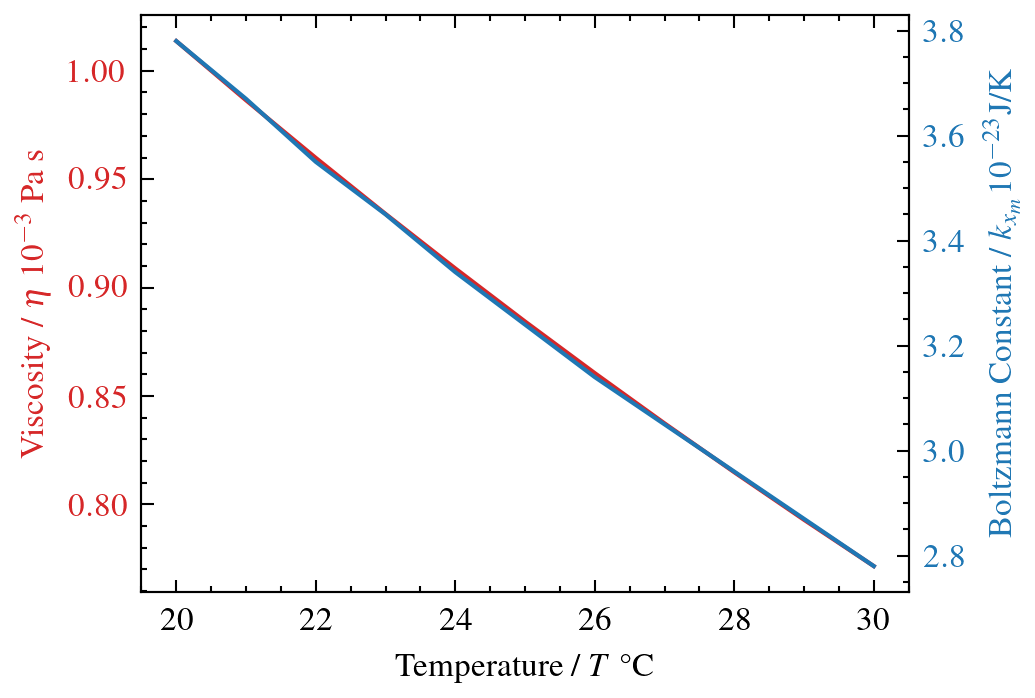
\includegraphics[keepaspectratio, width=\linewidth]{src/figures/k-n-relation/k-x-n-relation.png}
        \subcaption{$k_{x_m}$}
    \end{minipage}
    \begin{minipage}[b]{0.45\linewidth}
        \centering
        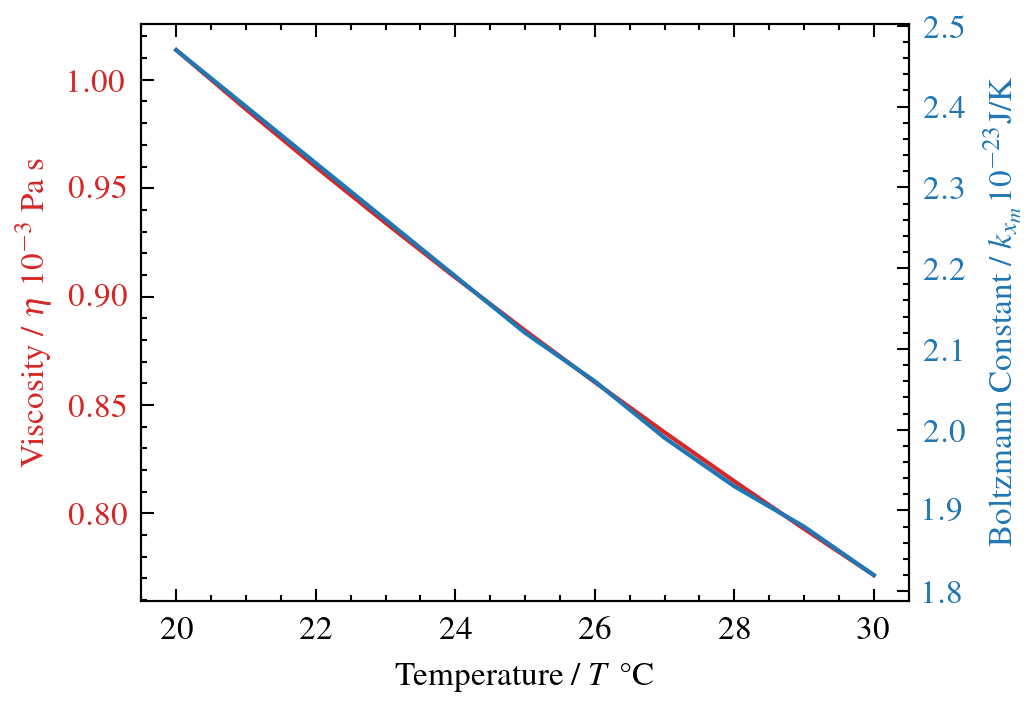
\includegraphics[width=\linewidth]{src/figures/k-n-relation/k-y-n-relation.png}
        \subcaption{$k_{y_m}$}
    \end{minipage}
    \caption{$k$と$\eta$の$T$依存性} \label{fig:k-n-relation}
\end{figure}


実際に計測された室温は\SI{26.6}{\celsius}で、
この周辺で$\eta$はほぼ線形で、同様に$k$も線形であると考えられる。
グラフから温度が\SI{1}{\celsius}異なると、
$\eta$はおよそ\SI{0.025}{\milli\pascal\second}変化している。
$k_{m_x}$は、\SI{0.07E-23}{\joule\per\kelvin}、
$k_{m_y}$は、\SI{0.06E-23}{\joule\per\kelvin}変化している。
したがって、十分長い時間溶液は放置され室温に近い温度になっていたとすれば、
温度の誤差は高々\SI{1}{\celsius}であるとして、
$k_{x_m}$、$k_{y_m}$の誤差はそれぞれ
$\SI{0.07E-23}{\joule\per\kelvin}$、$\SI{0.06E-23}{\joule\per\kelvin}$であると考えられる。

次に、$k$の$\ev{(\Delta x)^2}$依存性を考える。
式\ref{eq:brownian-motion}からわかる様に、$k$は$\ev{(\Delta x)^2}$に比例する。
これを図示すると、次の図\ref{fig:k-x-relation}のようになる。
このグラフから、$k$の理論値に対する$\ev{(\Delta x)^2}$は\SI{1.64}{\micro\meter\squared}であると計算できる。

$k_{x_m}$の相対誤差は\SI{57.5}{\percent}で2.35倍、
$k_{y_m}$の相対誤差は\SI{34.9}{\percent}で1.54倍であると計算できる。
よって本実験では、粒子のブラウン運動が理論値に比べて大きくランダムに運動していたとわかる。


\begin{figure}
    \centering
    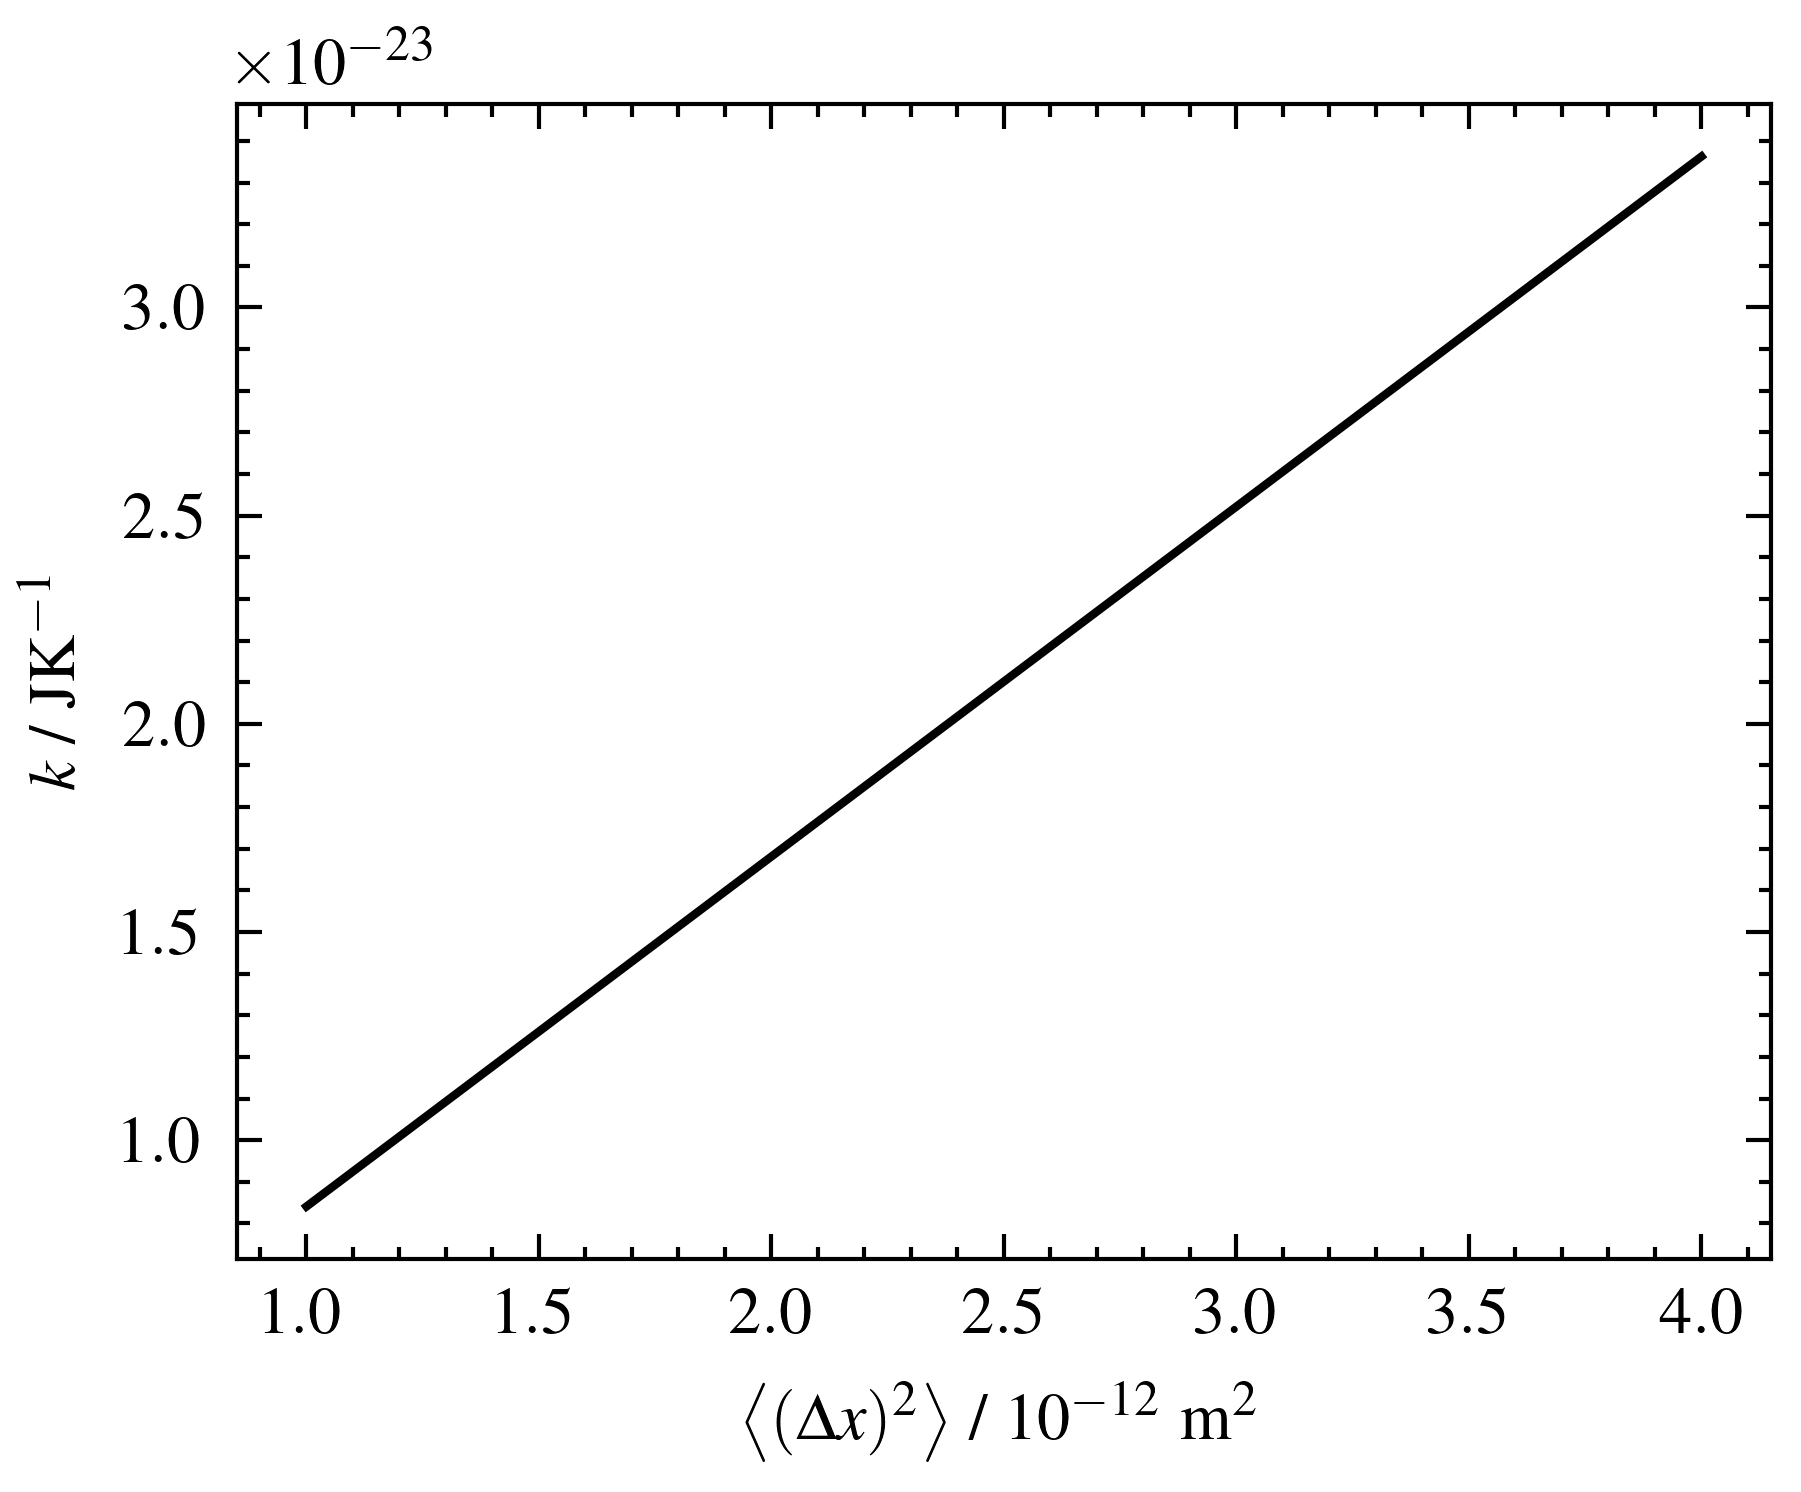
\includegraphics[keepaspectratio, width=0.8\linewidth]{src/figures/k-x-relation/k-x-relation.png}
    \caption{$k$と位置の移動量の分散$\ev{(\Delta x)^2}$の関係}\label{fig:k-x-relation}
\end{figure}

